\chapter{Introduction}
%Your report should start with an introduction chapter that motivates the subject in general and describes the problem you are trying to solve. 
%TODO:
The goals for the work on this term project was to give us experience with implementation of algorithms in hardware, verification by simulation, synthesis tools and to understand and evaluate other people's work by a peer-review system. \cite{ggmanual}.\cite{rsahardware}
\section{Problem Description and Analysis} % TODO: move this section to intro?

%- Describe the problem you are trying to solve?\\
%- What are the main requirements?\\
%- What do you need to investigate further before proposing a solution?\\

The task was to design and implement in hardware a RSA encryption/decryption circuit that meets the requirements listed in figure \ref{fig:req}. The message blocks to be encrypted are be 128-bit wide, and divided into four packets for transmission via a 32-bit wide parallell data bus into the circuit using a communication protocol as described in figure \ref{fig:interface}. 
\begin{figure}[H]
\centering
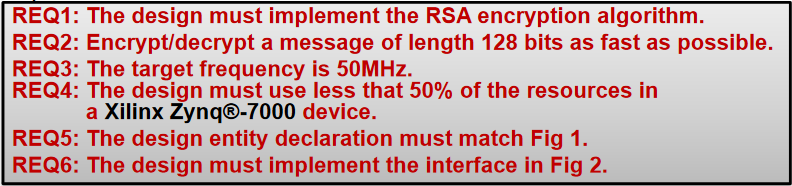
\includegraphics[width=0.7\textwidth]{images/requierements.PNG}
\caption{Design specification}
\label{fig:req}
\end{figure}
\begin{figure}[H]
\centering
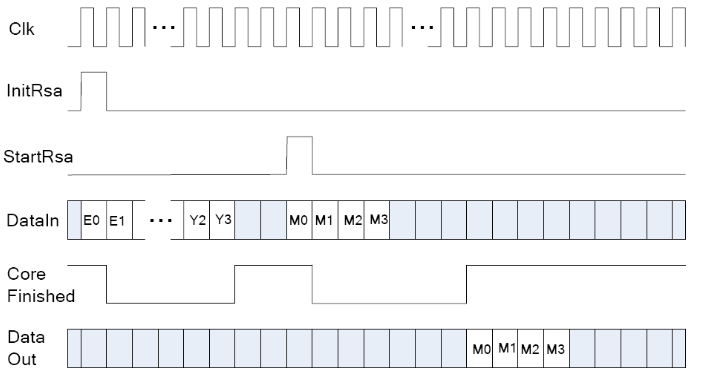
\includegraphics[width=0.7\textwidth]{images/communication.PNG}
\caption{Interface communication protocol}
\label{fig:interface}
\end{figure}

As part of the process, the RSA-module first has to be configured with the correct keys (this is the \emph{init} phase), where each key consists of two 128-bit integers before performing encryption or decryption on one or more message blocks.
